\section{Agent 批量推理中的中期抖动}
\label{sec:motivation}

Agent 批量推理呈现出与传统批量 LLM 服务显著不同的系统行为。本节揭示并刻画一种由 GPU 显存受限条件下 Agent 异步推进所诱发的现象，即\textit{中期抖动}，并说明其为何会在高并发下导致灾难性的吞吐崩塌。我们先通过简化的工作流示例解释其根因，再用真实部署中的经验测量加以验证。

\subsection{Agent 级异步性与 KV 缓存竞争}

图~\ref{fig:twoagent}a 展示了多个 Agent 共享有限 GPU 驻留 KV 缓存槽的情形。当 Agent 1 与 Agent 2（A1 和 A2）暂停去执行工具调用时，它们对应的 KV 缓存槽就暂时变为不活跃状态。按照标准 LRU 淘汰策略，这些条目会失去“最近访问”的优势，并在 Agent 3（A3）继续生成、不断占用内存时，首先成为淘汰对象。

因此，当暂停的 Agent（A1 与 A2）恢复执行时，服务引擎必须通过 prefill 重计算来重建整个前缀，这会带来显著时延。这个例子只是最简单的两方竞争情形。在存在大量 Agent 的系统中，随着各个 Agent 在主动生成和工具暂停之间反复切换，这类相互淘汰和重计算事件会更加频繁地发生。最终，级联式淘汰会在 Agent 执行的中段形成持久的缓存抖动，并演化为我们所说的\emph{中期抖动}。

\begin{figure}[tb]
    \centering
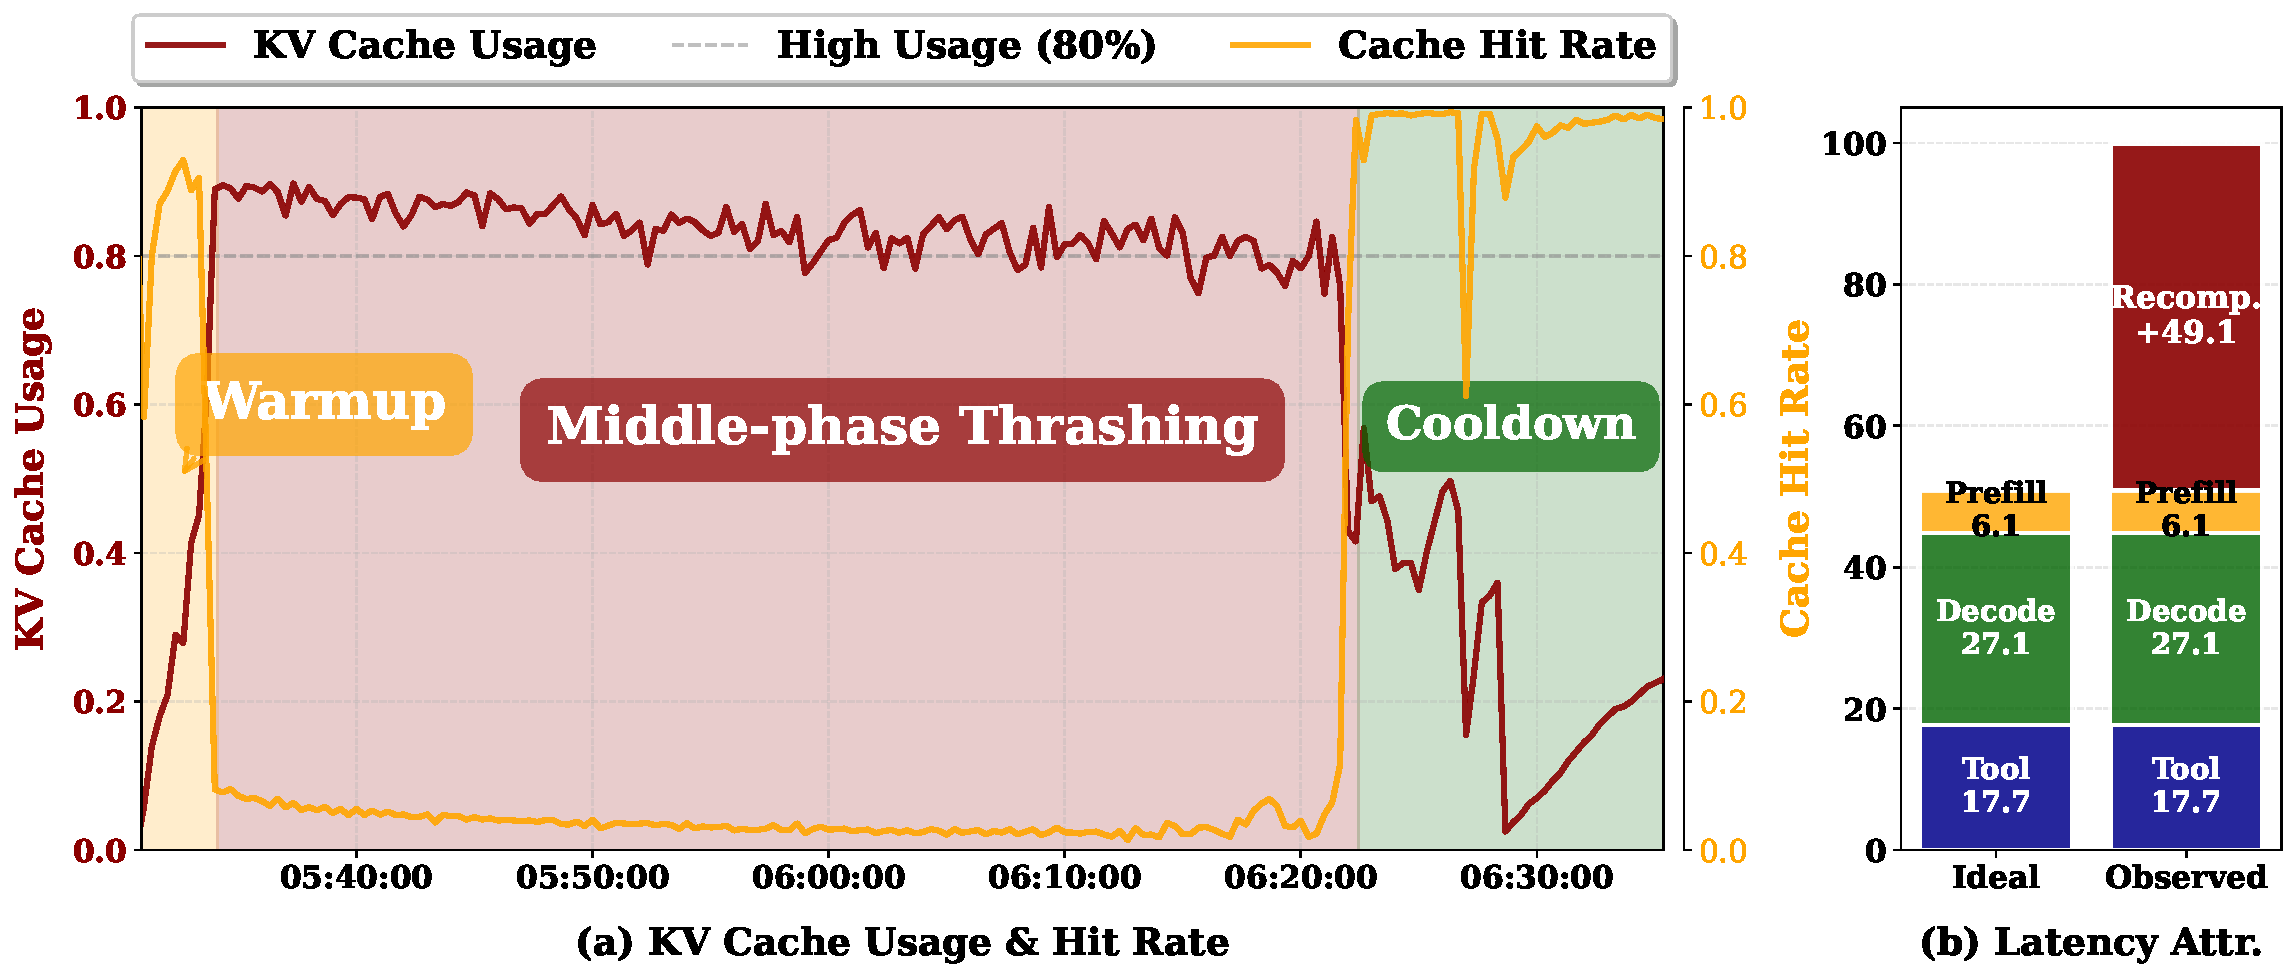
\includegraphics[width=0.98\linewidth]{figure/combined_figure.pdf}
\caption{\textbf{真实 Agent 批量推理中的中期抖动。}(a) 在 DeepSeek-V3 上运行基准测试时，端到端 KV 缓存占用随时间的演化。轨迹显示出 Agent 批量推理中典型的三阶段执行模式。(b) 同一次运行的端到端时延分解，展示 prefill、decode 与中期由 KV 缓存抖动引入的额外重计算开销所占比例。}
\label{fig:dpskthrashing}
\end{figure}

\subsection{通过经验分析刻画中期抖动}
\label{subsec:character-middle-phase}

为了理解 Agent 批量推理的资源动态，我们分析了高并发条件下基于 DeepSeek-V3 的大规模 Agent 部署执行轨迹。图~\ref{fig:dpskthrashing} 给出了聚合 GPU KV 缓存使用率与对应缓存命中率的时间序列。结果表明，Agent 工作负载的资源消耗并非均匀分布，而是遵循一种具有代表性的三阶段模式，其主导现象正是\textbf{中期抖动}。

(1) \noindent\textbf{预热阶段。} 在初始执行阶段（图~\ref{fig:dpskthrashing} 中的黄色区域），Agent 仍处于较浅的推理深度，上下文较短，且提示前缀高度共享。因此，KV 缓存占用较小、相似性高，服务引擎可以最大化前缀共享，命中率接近 90\%。在这个阶段，随着并发提升，吞吐通常会单调增加，因为整体工作集仍然远低于显存上限。

(2) \noindent\textbf{伴随抖动的中期阶段。} 随着 Agent 推进到中等长度的执行步骤，系统进入持续时间很长的中期抖动阶段，其耗时超过总执行时间的 90\%。从图~\ref{fig:dpskthrashing} 可以看到一个关键病态：KV 缓存占用始终维持在高位（大约 80\% 到 100\%），但缓存命中率却快速下降并长期维持在低位。持续低命中率说明系统并不是在“有效使用”显存，而是陷入了不断淘汰与重计算的循环。我们观察到，这部分额外重计算在完整生命周期中占到端到端时延的 49.1\%，与 prefill、decode 和工具调用等其他阶段相比占比极高。在这一阶段继续增加并发，反而会进一步恶化吞吐。

(3) \noindent\textbf{冷却阶段。} 最终，当部分 Agent 完成工作流并释放内存后，整体压力下降，淘汰频率降低，缓存命中率开始回升，系统逐渐退出抖动状态。

这些观察说明，在高吞吐 Agent 服务场景中，主要瓶颈并非峰值显存容量本身，而是现有内存管理在高度波动的中期阶段仍然采取被动策略。

\subsection{对系统设计的启示}

中期抖动的普遍存在揭示了当前 LLM 服务栈中的一个根本抽象失配。现有服务引擎采用请求级调度，将每一步生成都视为独立、无状态的工作单元。对于标准聊天补全任务，这种抽象是有效的；但对于 Agent 工作流，它无法表达跨多轮执行的长期状态连续性。

因此，我们认为系统设计必须沿两个维度完成范式转变：一是从请求级调度粒度转向 Agent 级调度粒度；二是从被动淘汰转向主动准入控制。这两条原则共同驱动了 \SysName{} 的设计，下一节将详细展开。
